\chapter{软件环境及设置}

该模版是基于CTeX社区发行的ctexbook模版,因此要使用该模版需要有CTeX环境。

与第一版稍有不同的时,由于该版提供了采用UTF-8编码的\XeTeX{}引擎的新版本和使用原有采用GBK编码的\LaTeX{}引擎的老版本,
因此,如果使用新版本,还需要参考本模版文件包中提供的ctex-xecjk-winfonts.def文件将自己系统中的
ctex-xecjk-winfonts.def文件进行修改,
该文件位于ctex目录下的$\backslash$tex$\backslash$latex$\backslash$ctex$\backslash$fontset目录下。
需要至少指定以下六种字体对应的字体文件:
\begin{verbatim}
\setCJKfamilyfont{zhsong}{SimSun}
\setCJKfamilyfont{zhhei}{SimHei}
\setCJKfamilyfont{zhkai}{KaiTi}
\setCJKfamilyfont{zhfs}{FangSong}
\setCJKfamilyfont{zhli}{LiSu}
\setCJKfamilyfont{zhyou}{YouYuan}

\newcommand*{\songti}{\CJKfamily{zhsong}} % 宋体
\newcommand*{\heiti}{\CJKfamily{zhhei}}   % 黑体
\newcommand*{\kaishu}{\CJKfamily{zhkai}}  % 楷书
\newcommand*{\fangsong}{\CJKfamily{zhfs}} % 仿宋
\newcommand*{\lishu}{\CJKfamily{zhli}}    % 隶书
\newcommand*{\youyuan}{\CJKfamily{zhyou}} % 幼圆
\end{verbatim}

其它字体可以自由指定,SimSun,SimHei这些指定字体的关键字可以直接用字体文件*.ttf 来代替,
也可以使用命令“fc-list”来具体查看系统中已安装的字体的名字,从而对应地填到上述命令中去。

2015年年底的时,CteX推出了2.X版,这个版本对系统中存在的字体的自动判断以及加载已比较完善,一般情况已不需要专门调整设置了。只要保证系统中存在这六种字体的文件即可,这其中尤其要{\bfseries 注意}的是隶书与幼圆两个字体不是Winddows自带而是Office自带字体,没有安装Office的电脑需要把这两个字体拷到Windows 下的Font文件夹中去。


\section{Microsoft Windows系统}

Windows系统下可以直接安装CTeX发行的软件包,该发行包只有32位版本,64位系统安装方法与32位略有不同。下面分别介绍。

\subsection{32位系统}

包括windows XP,Windows Server 2003,Vista, Windows Server 2008 和 Windows 7。

32位系统下安装比较简单,直接从www.ctex.org下载最新的安装包,当前最新版为2.9.0.152,
它包括CTeX环境,winEdt,MiKTeX,Ghostcript,几个部分,除CTeX环境外,
另外几个组件都可以选择安装,如可以用TeXLive替代MiKTeX,UltraEdit,gvim,Emacs替代winEdit等。
如果你不了解这几个软件,那么就默认安装选项即可。

安装完后,需要对\LaTeX 软件进行升级,如MiKTeX软件进行升级,升级的网络站点就选中科大的CTAN镜像站,
网址http://mirrors.ustc.edu.cn/CTAN,在教育网内速度还是比较快的,如图\ref{set1},\ref{set2},\ref{set3}所示。

\begin{figure}[th]
\centering
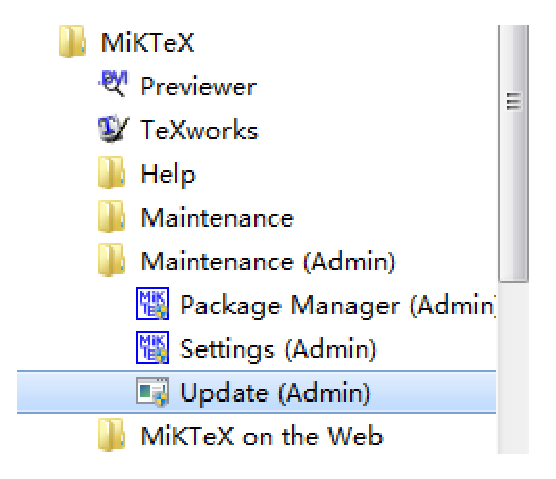
\includegraphics[scale=0.5]{./Pictures/set1.eps}\\
\caption{MiKTeX升级设置}
\label{set1}
\end{figure}

\begin{figure}[th]
\centering
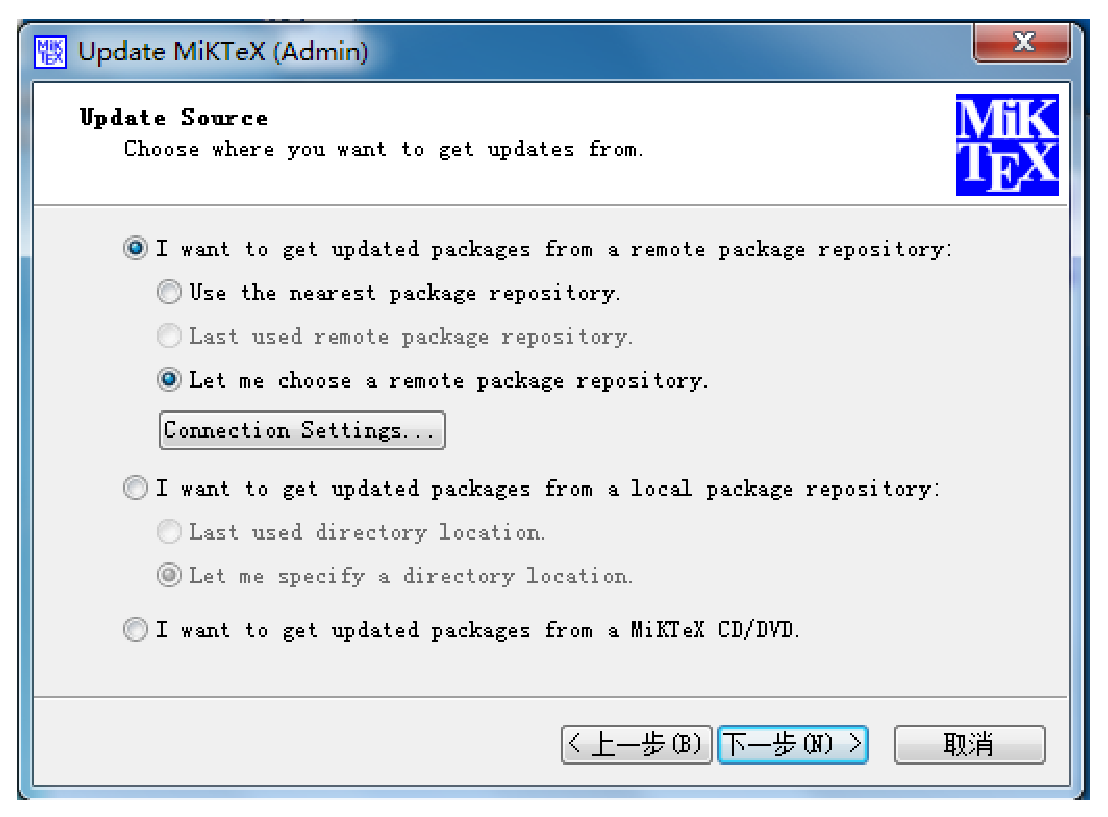
\includegraphics[scale=0.5]{./Pictures/set2.eps}\\
\caption{选择升级方式,如图中选择一个升级站点}
\label{set2}
\end{figure}

\begin{figure}[th]
\centering
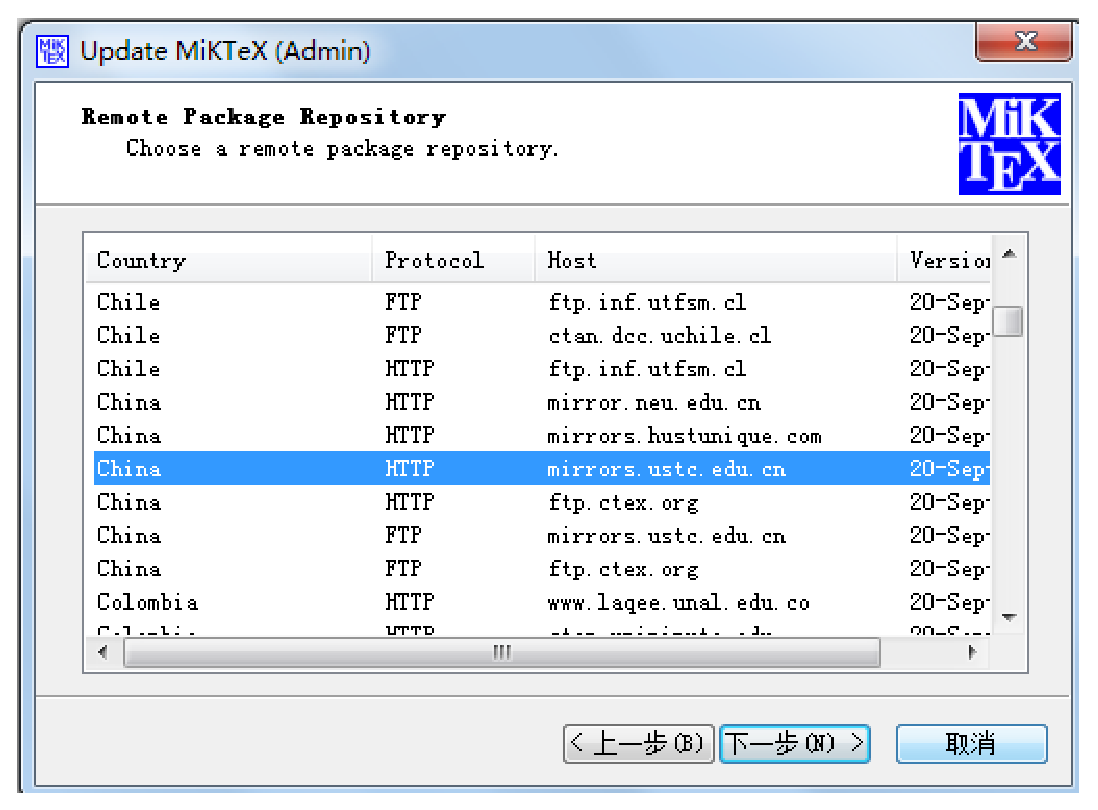
\includegraphics[scale=0.5]{./Pictures/set3.eps}\\
\caption{选择升级站点,以中科大镜像点为例}
\label{set3}
\end{figure}

之所以要把软件升级到最新是因为该模版使用了最新的hyperref包中添加的命令hidelinks。

\subsection{64位系统}

包括windows XP 64bit,Windows Server 2003 64bit,Vista 64bit,
Windows Server 2008 64bit,Windows 7 64bit 和 Windows Server 2008 R2。
当然现在还有了Windows 8,Windows 8.1和Windows 10。

安装CTeX安装包时,不要选择MiKTeX,其它软件任意,与32位一样。
安装完CTeX包后,去www.miktex.org网站下载MiKTeX的最新64位版,当前是2.9版,

安装后不需要进行特殊的设置,现在的CTeX功能包已经是latex扩展库中的一部分,
可以直接通过发行版自带的包管理系统下载安装该功能包。如图\ref{Roots}所示,在设置界面中的Root设置留空即可。

\begin{figure}[th]
	\centering
	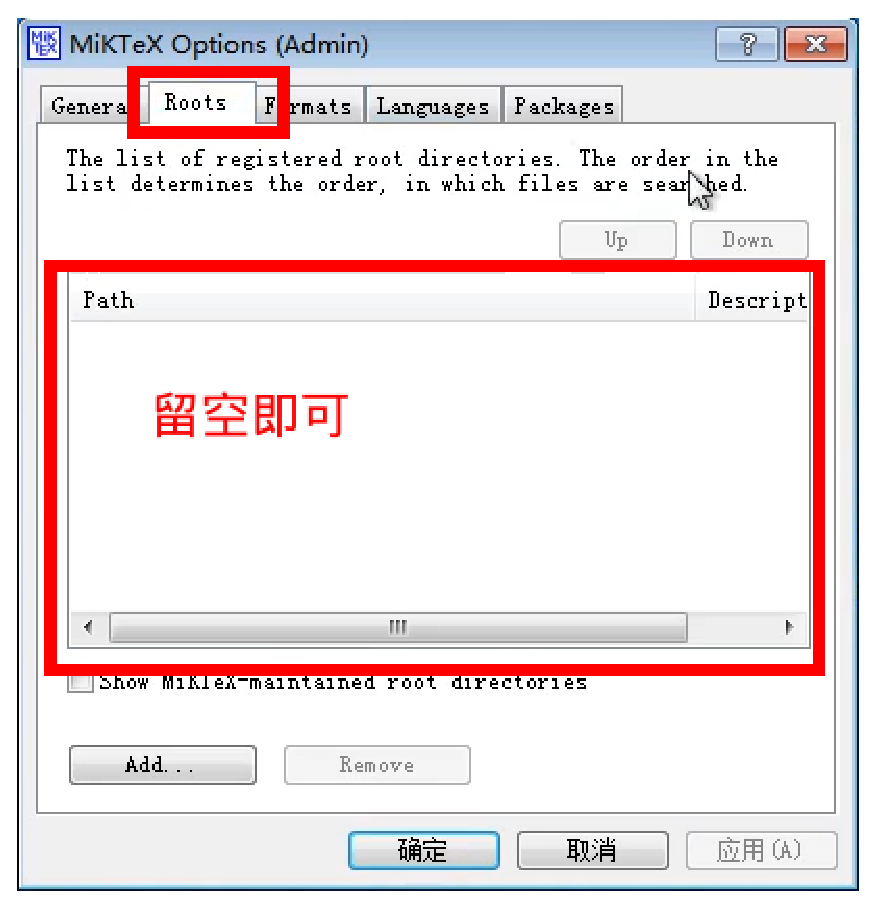
\includegraphics[scale=0.5]{./Pictures/Roots.eps}\\
	\caption{MiKTeX的Roots设置}
	\label{Roots}
\end{figure}

与32位Windows系统相同,安装完后也需要把MiKTeX升级到最新。

\section{linux系统}

请自行选择\LaTeX 安装版本,然后把CTeX环境加入即可。我想用linux的应该都会这个吧。
本次版本使用的操作系统及软件环境是ubuntu 14.04和TeXLive2014。

请保证扩展包版本足够新。尤其是hyperref包,保证是2011年8月份后的版本。

\section{Mac系统}

请自行选择\LaTeX 安装版本,加入CTeX环境。同linux下方法。一般是TeXLive,
通过其自带的包管理加载所需要的功能扩展包。

\section{本模版所需要的扩展包}

\begin{enumerate}

\item{图形、表格类扩展包} graphicx,array,booktabs,caption,natbib,multirow

\item{字体类扩展包} times(\LaTeX{}引擎中用),fontspec(\XeTeX{}引擎中用)

\item{目录选项扩展包} tocbibind,tocloft,makeidx,hyperref

\item{数学公式扩展包} amsmath,amsthm,amsfonts,amssymb,bm

\end{enumerate}

\section{测试运行}

如果已经安装好了CTeX环境与\LaTeX 软件,那么,可以运行这个模版文件包里的makethesis.bat文件,
几秒钟到十几秒后,如果生成了一份叫做“论文模版示例.pdf”的文档,那么,恭喜,这个模版所需要的软件环境建立成功!
如果没有生成这一份文件,那么有可能你的软件环境没有配置正确,比如把\LaTeX 软件升级到最新,
这份模版所需要的扩展包没有被安装,请打开\LaTeX 软件自动升级功能,
保证\LaTeX 软件能够成功地连接到CTAN站点下载所需的扩展功能包。

以Windows 系统gbk版本为例,具体测试运行过程如下:

打开cmd命令行工具,进入该模版所在目录,输入\LaTeX 命令如图\ref{runbat} 所示:

\begin{figure}[th]
	\centering
	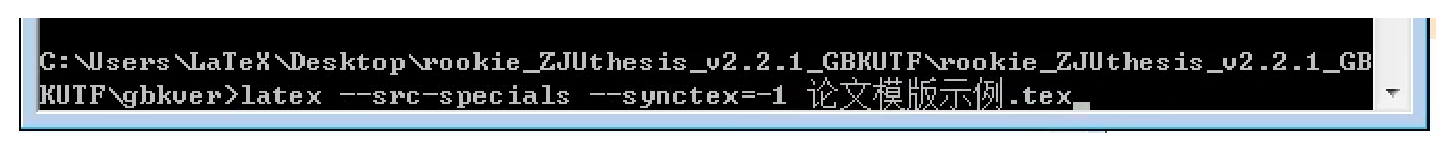
\includegraphics[scale=0.5]{./Pictures/runbat.eps}\\
	\caption{cmd窗口中运行\LaTeX 命令}
	\label{runbat}
\end{figure}

如果系统中MiKTeX的扩展包未安装完全,可能会弹出如图\ref{SelRep}所示窗口。
点“Change”按钮选择一个网络安装源。如果不选择就是由系统随机选择一个源(Random package repository)。

\begin{figure}[th]
	\centering
	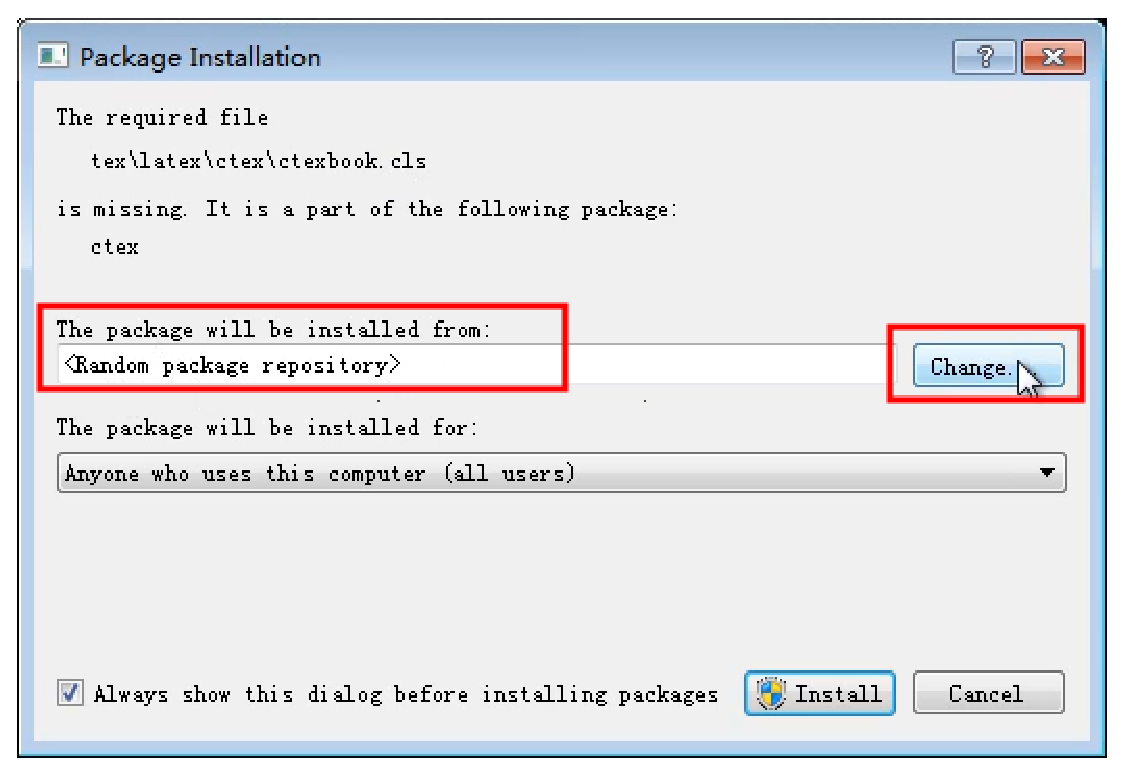
\includegraphics[scale=0.5]{./Pictures/SelRep.eps}\\
	\caption{下载缺少的扩展功能包}
	\label{SelRep}
\end{figure}

\newpage

点了"Change"按钮之后,在如图\ref{PkgInternet}所示界面中选择从网络源上下载。

\begin{figure}[th]
	\centering
	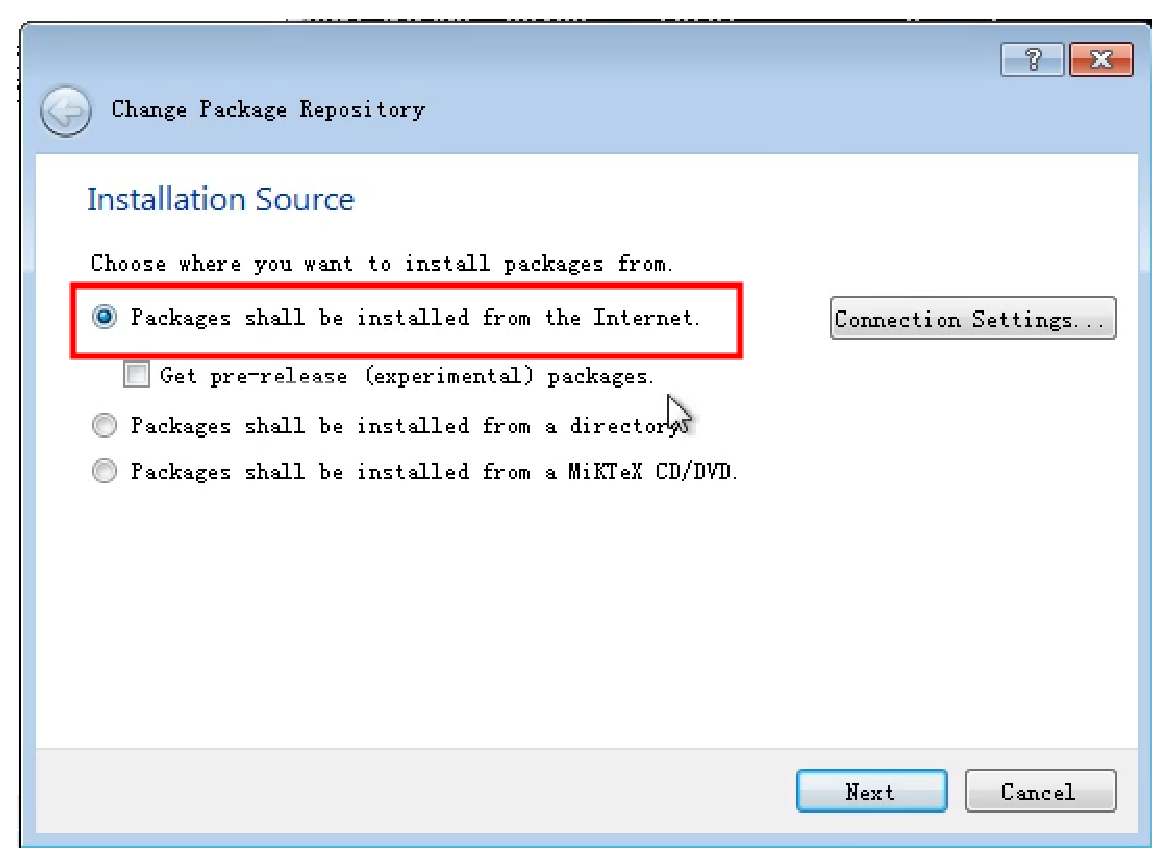
\includegraphics[scale=0.5]{./Pictures/PkgInternet.eps}\\
	\caption{选择网络源}
	\label{PkgInternet}
\end{figure}

下一步,选择一个源,最好是国内的源,速度比较快,如图\ref{SelRep_0}所示。
推荐使用HTTP协议,用FTP协议的站容易连接失败。

\begin{figure}[th]
	\centering
	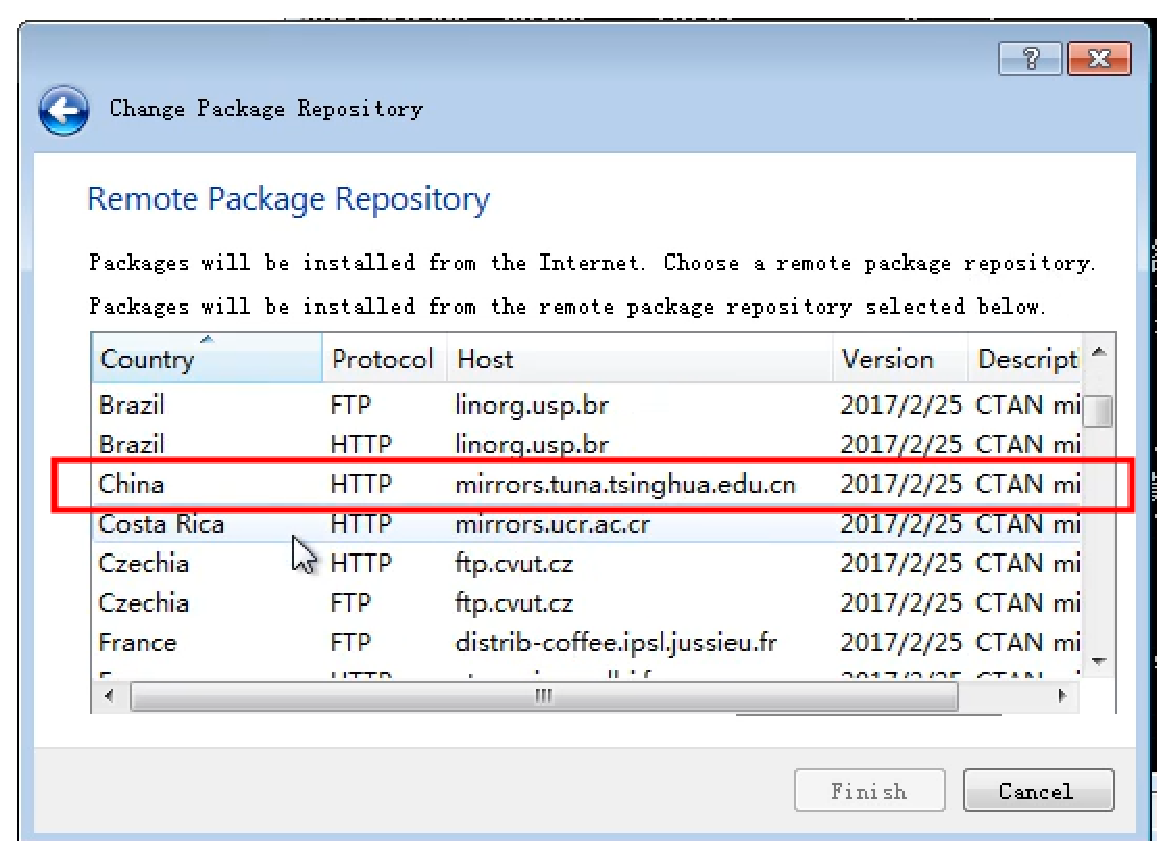
\includegraphics[scale=0.5]{./Pictures/SelRep_0.eps}\\
	\caption{选择国内安装源}
	\label{SelRep_0}
\end{figure}

\newpage

选择好之后,按“Install”按钮。如图\ref{PkgSelect}所示。

\begin{figure}[th]
	\centering
	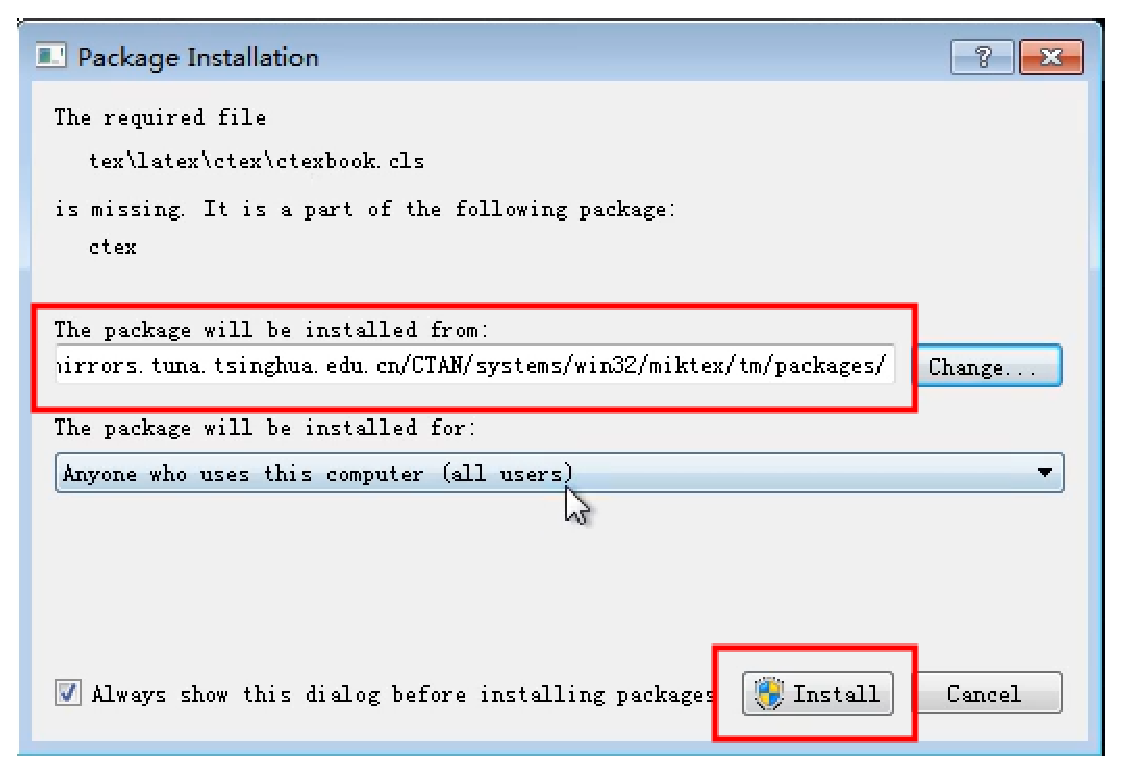
\includegraphics[scale=0.5]{./Pictures/PkgSelect.eps}\\
	\caption{选择好之后安装}
	\label{PkgSelect}
\end{figure}

按下安装之后,即可下载缺失包。如图\ref{Download}所示。

\begin{figure}[th]
	\centering
	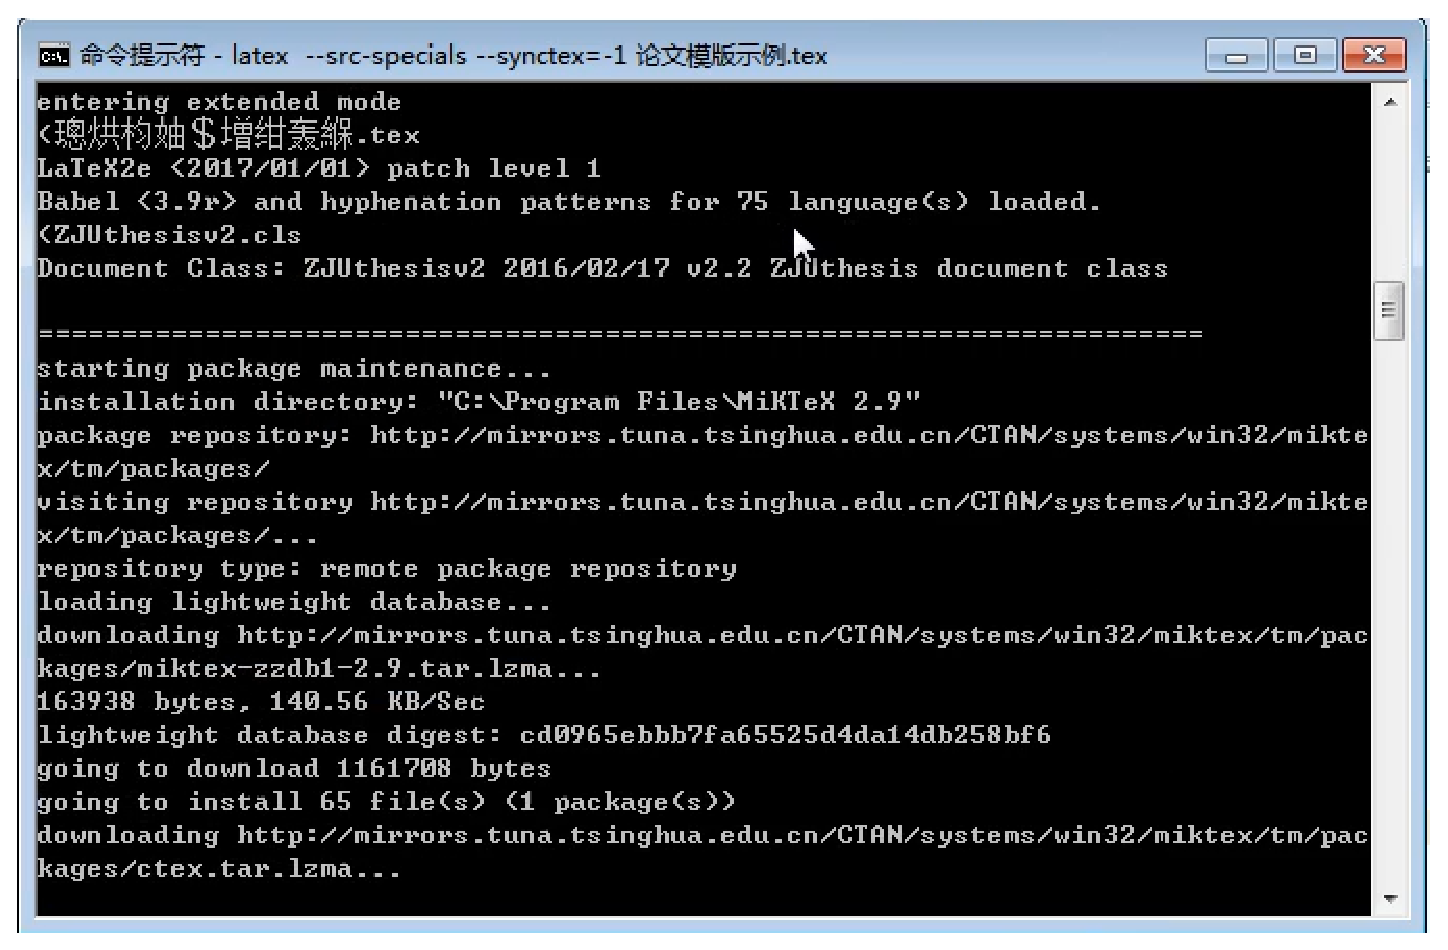
\includegraphics[scale=0.5]{./Pictures/Download.eps}\\
	\caption{选择好源后,下载过程中}
	\label{Download}
\end{figure}

\newpage

但这样每缺一个包,就会提示一次,这样会比较烦,可以把下面这个选择点掉,再按“Install”按键。

\begin{figure}[th]
	\centering
	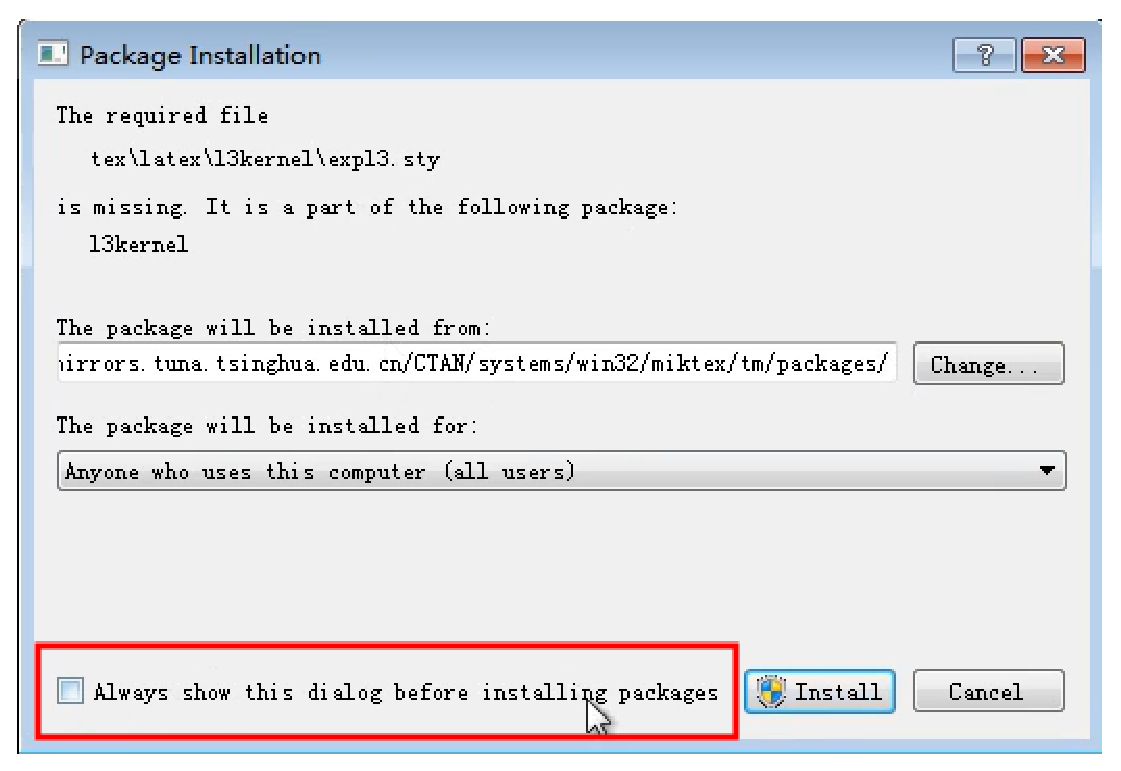
\includegraphics[scale=0.5]{./Pictures/NoShow.eps}\\
	\caption{点掉每次提示的选项}
	\label{NoShow}
\end{figure}

持续自动下载缺失的包如图\ref{l3kernel}所示。

\begin{figure}[th]
	\centering
	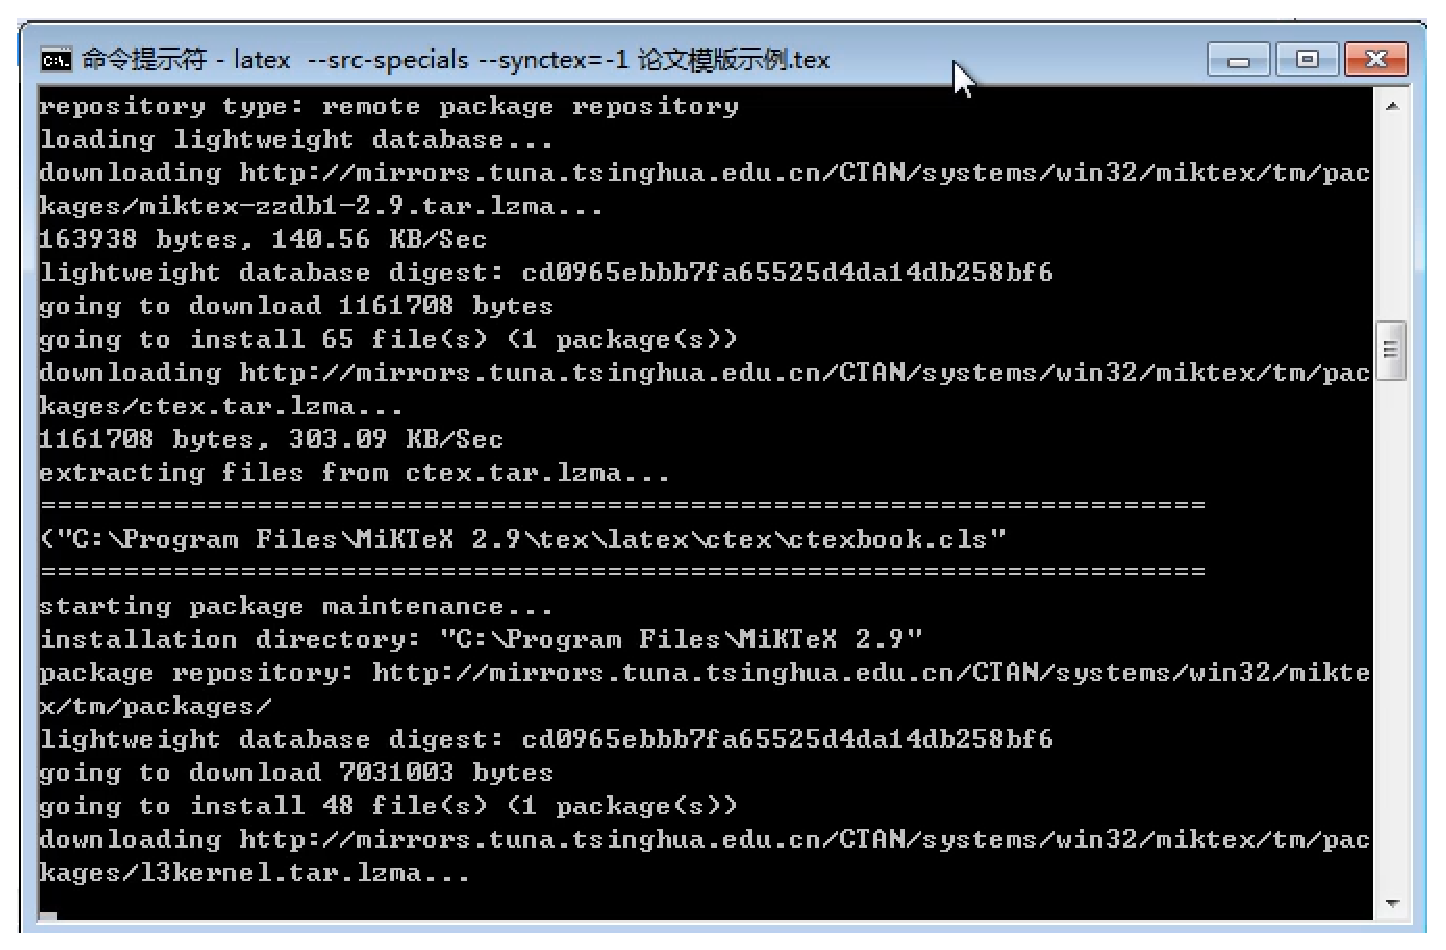
\includegraphics[scale=0.5]{./Pictures/l3kernel.eps}\\
	\caption{持续自动下载缺失的扩展包}
	\label{l3kernel}
\end{figure}

\newpage

\LaTeX 运行完成后,需要将生成的dvi转换为pdf,运行dvipdfmx进行转换。这个地方要提一点的是,
如果系统中字体没有安装完全, 比如隶书与幼圆字体没有安装,就会出现如图\ref{dvierror}所示的错误提示。

\begin{figure}[th]
	\centering
	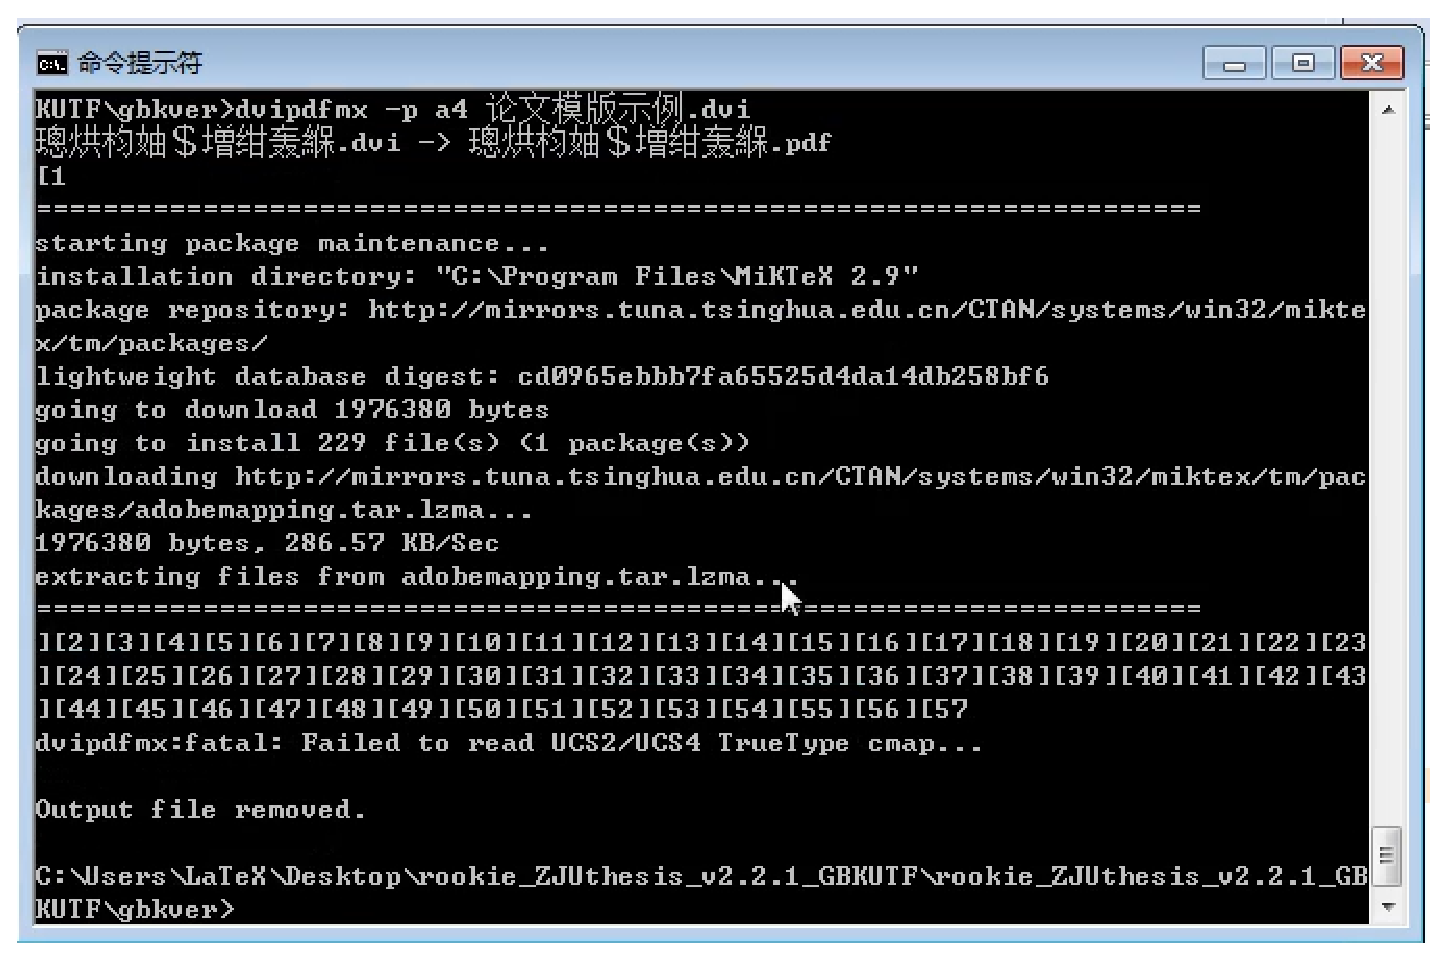
\includegraphics[scale=0.5]{./Pictures/dvierror.eps}\\
	\caption{转换pdf时可能出现的错误}
	\label{dvierror}
\end{figure}

将缺失的隶书与幼圆字体装入系统后,正常运行输出了pdf,如图所示。

\begin{figure}[th]
	\centering
	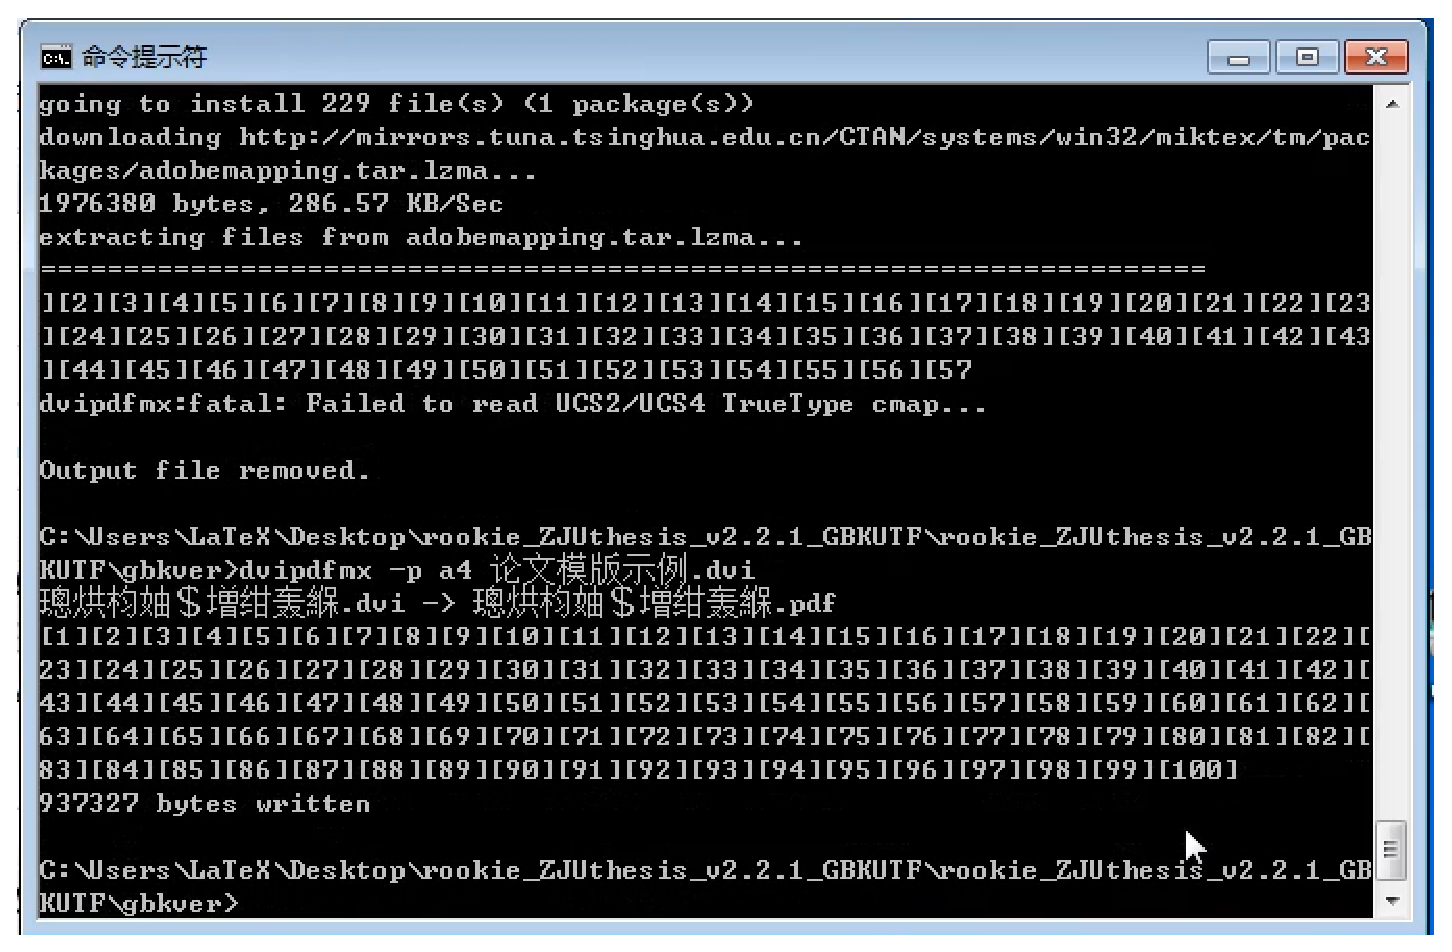
\includegraphics[scale=0.5]{./Pictures/complete.eps}\\
	\caption{生成pdf成功}
	\label{complete}
\end{figure}

使用\XeTeX 的utf版的使用过程与上述gbk版的过程类似,中间也会下载一些缺失的扩展包。